% answers.tex —— 2011 年·上海春季卷 · 参考答案与详细解析片段
% 由 tools/generate_projects.py 依来源总账自 2011/2011_数学真题_上海春季_试题.md + 2011/2011_数学真题_上海春季_解析正文.md + 2011/2011_数学真题_上海春季_答案要点.md 生成，勿手改（改源 MD 后重跑）

\begin{answer}
\gksolhead{1}{}

\textbf{题目}：

函数 $y=\lg(x-2)$ 的定义域是\gkblank{}。

\Needspace{4\baselineskip}
\textbf{解析}
对数的真数须为正：$x-2>0$，故定义域为 $(2,+\infty)$。

\gkanswer{答案：$(2,+\infty)$。}

\end{answer}
\begin{answer}
\gksolhead{2}{}

\textbf{题目}：

若集合 $A=\{x\mid x\geqslant1\}$，$B=\{x\mid x^2\leqslant4\}$，则 $A\cap B=$\gkblank{}。

\Needspace{4\baselineskip}
\textbf{解析}
$x^2\leqslant4$ 即 $-2\leqslant x\leqslant2$，故 $B=[-2,2]$。与 $A=[1,+\infty)$ 取交集得 $A\cap B=[1,2]=\{x\mid1\leqslant x\leqslant2\}$。

\gkanswer{答案：$\{x\mid1\leqslant x\leqslant2\}$。}

\end{answer}
\begin{answer}
\gksolhead{3}{}

\textbf{题目}：

在 $\triangle ABC$ 中，若 $\tan A=\dfrac{\sqrt2}3$，则 $\sin A=$\gkblank{}。

\Needspace{4\baselineskip}
\textbf{解析}
\Needspace{5\baselineskip}
$\tan A=\dfrac{\sqrt2}3>0$，故 $A$ 为锐角，
\nopagebreak[4]
\[\sin A=\frac{\tan A}{\sqrt{1+\tan^2A}}=\frac{\sqrt2/3}{\sqrt{1+2/9}}=\frac{\sqrt2}{\sqrt{11}}=\frac{\sqrt{22}}{11}.\]

\gkanswer{答案：$\dfrac{\sqrt{22}}{11}$。}

\end{answer}
\begin{answer}
\gksolhead{4}{}

\textbf{题目}：

若行列式 $\begin{vmatrix}2^x&4\\ 1&2\end{vmatrix}=0$，则 $x=$\gkblank{}。

\Needspace{4\baselineskip}
\textbf{解析}
\nopagebreak[4]
\[\begin{vmatrix}2^x&4\\ 1&2\end{vmatrix}=2^{x+1}-4=0\Longrightarrow2^{x+1}=2^2\Longrightarrow x=1.\]

\gkanswer{答案：$1$。}

\end{answer}
\begin{answer}
\gksolhead{5}{}

\textbf{题目}：

若 $\sin x=\dfrac13$，$x\in\left[-\dfrac\pi2,\dfrac\pi2\right]$，则 $x=$\gkblank{}。（结果用反三角函数值表示）

\Needspace{4\baselineskip}
\textbf{解析}
$x\in\left[-\dfrac\pi2,\dfrac\pi2\right]$ 时 $\sin$ 单调递增，故 $x=\arcsin\dfrac13$。

\gkanswer{答案：$\arcsin\dfrac13$。}

\end{answer}
\begin{answer}
\gksolhead{6}{}

\textbf{题目}：

$\left(x+\dfrac1x\right)^6$ 的二项展开式的常数项为\gkblank{}。

\Needspace{4\baselineskip}
\textbf{解析}
通项 $T_{k+1}=\mathrm C_6^kx^{6-k}\left(\dfrac1x\right)^k=\mathrm C_6^kx^{6-2k}$。令 $6-2k=0$ 得 $k=3$，常数项为 $\mathrm C_6^3=20$。

\gkanswer{答案：$20$。}

\end{answer}
\begin{answer}
\gksolhead{7}{}

\textbf{题目}：

两条直线 $l_1:x-\sqrt3y+2=0$ 与 $l_2:x-y+2=0$ 夹角的大小是\gkblank{}。

\Needspace{4\baselineskip}
\textbf{解析}
$l_1$ 的斜率为 $\dfrac1{\sqrt3}$，倾斜角 $30^\circ$；$l_2$ 的斜率为 $1$，倾斜角 $45^\circ$。夹角为 $45^\circ-30^\circ=15^\circ=\dfrac\pi{12}$。

\gkanswer{答案：$\dfrac\pi{12}$。}

\end{answer}
\begin{answer}
\gksolhead{8}{}

\textbf{题目}：

若 $S_n$ 为等比数列 $\{a_n\}$ 的前 $n$ 项和，$8a_2+a_5=0$，则 $\dfrac{S_6}{S_3}=$\gkblank{}。

\Needspace{4\baselineskip}
\textbf{解析}
\Needspace{5\baselineskip}
$8a_2+a_5=0$ 即 $a_1q(8+q^3)=0$，故 $q^3=-8$，$q=-2$。于是
\nopagebreak[4]
\[\frac{S_6}{S_3}=\frac{1-q^6}{1-q^3}=1+q^3=1-8=-7.\]

\gkanswer{答案：$-7$。}

\end{answer}
\begin{answer}
\gksolhead{9}{}

\textbf{题目}：

若椭圆 $C$ 的焦点和顶点分别是双曲线 $\dfrac{x^2}{5}-\dfrac{y^2}{4}=1$ 的顶点和焦点，则椭圆 $C$ 的方程是\gkblank{}。

\Needspace{4\baselineskip}
\textbf{解析}
双曲线 $\dfrac{x^2}5-\dfrac{y^2}4=1$ 的顶点为 $(\pm\sqrt5,0)$，焦点为 $(\pm3,0)$。
椭圆 $C$ 的焦点是 $(\pm\sqrt5,0)$，顶点是 $(\pm3,0)$，故 $c=\sqrt5$，$a=3$，$b^2=9-5=4$，方程为 $\dfrac{x^2}9+\dfrac{y^2}4=1$。

\gkanswer{答案：$\dfrac{x^2}9+\dfrac{y^2}4=1$。}

\end{answer}
\begin{answer}
\gksolhead{10}{}

\textbf{题目}：

若点 $O$ 和点 $F$ 分别为椭圆 $\dfrac{x^2}{2}+y^2=1$ 的中心和左焦点，点 $P$ 为椭圆上的任意一点，则 $|OP|^2+|PF|^2$ 的最小值为\gkblank{}。

\Needspace{4\baselineskip}
\textbf{解析}
\Needspace{5\baselineskip}
椭圆 $\dfrac{x^2}2+y^2=1$ 中 $a=\sqrt2$，$b=1$，$c=1$，左焦点 $F(-1,0)$，中心 $O(0,0)$。设 $P(x,y)$，则
\nopagebreak[4]
\[|OP|^2+|PF|^2=x^2+y^2+(x+1)^2+y^2=2x^2+2x+1+2y^2.\]
\Needspace{5\baselineskip}
由 $y^2=1-\dfrac{x^2}2$ 得
\nopagebreak[4]
\[|OP|^2+|PF|^2=2x^2+2x+1+2-x^2=(x+1)^2+2.\]
$x\in[-\sqrt2,\sqrt2]$，当 $x=-1$ 时取最小值 $2$。

\gkanswer{答案：$2$。}

\end{answer}
\begin{answer}
\gksolhead{11}{}

\textbf{题目}：

根据如图所示的程序框图，输出结果 $i=$\gkblank{}。
\nopagebreak[4]
\begin{center}% 2011 年上海春季卷第 11 题：程序框图（i=0,s=66；s>0 时反复 s=s-10、i=i+1）
% 来源 PDF：春季高考/2011/2011春季上海.pdf，第 1 页（原刊 2-32 页）第 2 栏。
% 重绘依据：原图为「开始 → i=0,s=66 → 判断 s≤0?」，否分支向右执行 s=s-10、i=i+1 后
%   回到判断入口，是分支向下「输出 i」并「结束」。
\begin{tikzpicture}[scale=0.9, semithick, >=Stealth,
  block/.style={draw, minimum width=2.6cm, minimum height=0.7cm, align=center},
  dec/.style={draw, diamond, aspect=3.0, inner sep=1pt, align=center},
  arr/.style={->}]
  \node (start) [draw, rounded corners=6pt, minimum width=1.5cm, minimum height=0.55cm] {开始};
  \node (init)  [block, below=0.5cm of start] {$i=0,\ s=66$};
  \node (dec)   [dec, below=0.9cm of init] {$s\leqslant0$?};
  \node (out)   [draw, trapezium, trapezium left angle=70, trapezium right angle=110,
                 minimum width=2.4cm, minimum height=0.65cm, below=0.9cm of dec] {输出 $i$};
  \node (end)   [draw, rounded corners=6pt, minimum width=1.5cm, minimum height=0.55cm,
                 below=0.5cm of out] {结束};
  \node (sub)   [block, right=1.6cm of dec] {$s=s-10$};
  \node (add)   [block, above=0.7cm of sub] {$i=i+1$};
  \coordinate (join) at ($(init)!0.5!(dec)$);
  \draw[arr] (start) -- (init);
  \draw[arr] (init) -- (dec);
  \draw[arr] (dec) -- node[right] {是} (out);
  \draw[arr] (out) -- (end);
  \draw[arr] (dec.east) -- node[above] {否} (sub.west);
  \draw[arr] (sub.north) -- (add.south);
  \draw (add.west) -- (join -| add.west) -- (join);
  \draw[arr] (join -| add.west) -- (join);
\end{tikzpicture}
\end{center}
\nopagebreak[4]
\Needspace{4\baselineskip}
\textbf{解析}
初值 $i=0$，$s=66$。每次 $s>0$ 时执行 $i=i+1$，$s=s-10$。
经 $7$ 次：$s=66-70=-4\leqslant0$，此时 $i=7$，输出 $7$。

\gkanswer{答案：$7$。}

\end{answer}
\begin{answer}
\gksolhead{12}{}

\textbf{题目}：

2011 年上海春季高考有 8 所高校招生，如果某 3 位同学恰好被其中 2 所高校录取，那么录取方法的种数为\gkblank{}。

\Needspace{4\baselineskip}
\textbf{解析}
先从 $8$ 所高校中选出被录取的 $2$ 所，有 $\mathrm C_8^2=28$ 种；再把 $3$ 位同学安排到这 $2$ 所且两所都有人，有 $2^3-2=6$ 种。故共有 $28\times6=168$ 种。

\gkanswer{答案：$168$。}

\end{answer}
\begin{answer}
\gksolhead{13}{}

\textbf{题目}：

有一种多面体的饰品，其表面由 6 个正方形和 8 个正三角形组成（如图），$AB$ 与 $CD$ 所成角的大小是\gkblank{}。
\nopagebreak[4]
\begin{center}% 2011 年上海春季卷第 13 题：由 6 个正方形与 8 个正三角形组成的多面体（立方八面体），
% AB 与 CD 为其中两条棱。
% 来源 PDF：春季高考/2011/2011春季上海.pdf，第 1 页（原刊 2-32 页）第 2 栏。
% 重绘依据：原图为该多面体的线框图，实线为可见棱、虚线为被遮挡棱；
%   本图按顶点 (\\pm1,\\pm1,0) 的排列取斜投影，沿用原图实/虚线约定。
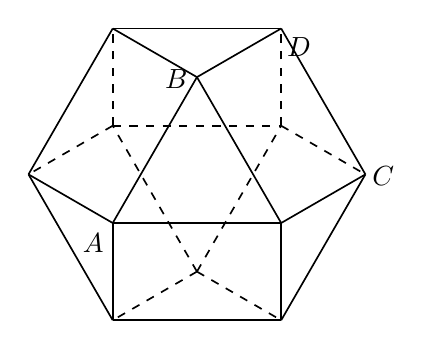
\begin{tikzpicture}[scale=0.95, semithick, every node/.style={inner sep=1.5pt}]
  % 可见棱
  \draw (-1.126,-1.950) -- (-2.252,0.000);
  \draw (-1.126,-1.950) -- (1.126,-1.950);
  \draw (-1.126,-1.950) -- (-1.126,-0.650);
  \draw (-2.252,0.000) -- (-1.126,1.950);
  \draw (-2.252,0.000) -- (-1.126,-0.650);
  \draw (1.126,-1.950) -- (2.252,0.000);
  \draw (1.126,-1.950) -- (1.126,-0.650);
  \draw (-1.126,1.950) -- (1.126,1.950);
  \draw (-1.126,1.950) -- (0.000,1.300);
  \draw (-1.126,-0.650) -- (1.126,-0.650);
  \draw (-1.126,-0.650) -- (0.000,1.300);
  \draw (2.252,0.000) -- (1.126,1.950);
  \draw (2.252,0.000) -- (1.126,-0.650);
  \draw (1.126,1.950) -- (0.000,1.300);
  \draw (1.126,-0.650) -- (0.000,1.300);
  % 被遮挡棱
  \draw[dashed] (0.000,-1.300) -- (-1.126,0.650);
  \draw[dashed] (0.000,-1.300) -- (-1.126,-1.950);
  \draw[dashed] (0.000,-1.300) -- (1.126,0.650);
  \draw[dashed] (0.000,-1.300) -- (1.126,-1.950);
  \draw[dashed] (-1.126,0.650) -- (-2.252,0.000);
  \draw[dashed] (-1.126,0.650) -- (1.126,0.650);
  \draw[dashed] (-1.126,0.650) -- (-1.126,1.950);
  \draw[dashed] (1.126,0.650) -- (2.252,0.000);
  \draw[dashed] (1.126,0.650) -- (1.126,1.950);
  % 标注：A=(0,1,1)、B=(1,1,0)、C=(1,-1,0)、D=(1,0,-1) 四个顶点
  \node[below left]  at (-1.18,-0.72) {$A$};
  \node[left]        at (-0.06,1.28) {$B$};
  \node[right]       at (2.28,-0.02) {$C$};
  \node[below right] at (1.14,1.90) {$D$};
\end{tikzpicture}
\end{center}
\nopagebreak[4]
\Needspace{4\baselineskip}
\textbf{解析}
该多面体由 $6$ 个正方形与 $8$ 个正三角形组成，是立方八面体。取坐标系使各顶点为 $(\pm1,\pm1,0)$、$(\pm1,0,\pm1)$、$(0,\pm1,\pm1)$ 的排列。
\Needspace{5\baselineskip}
$AB$ 与 $CD$ 是其中的两条棱，可取 $A(0,1,1)$，$B(1,1,0)$，$C(1,-1,0)$，$D(1,0,-1)$，于是
\nopagebreak[4]
\[\overrightarrow{AB}=(1,0,-1),\qquad\overrightarrow{CD}=(0,1,-1),\]
\nopagebreak[4]
\[\cos\langle\overrightarrow{AB},\overrightarrow{CD}\rangle=\frac{0+0+1}{\sqrt2\cdot\sqrt2}=\frac12,\]
故两棱所成角为 $\dfrac\pi3$。

\gkanswer{答案：$\dfrac\pi3$。}

\end{answer}
\begin{answer}
\gksolhead{14}{}

\textbf{题目}：

为求解方程 $x^5-1=0$ 的虚根，可以把原方程变形为 $(x-1)(x^4+x^3+x^2+x+1)=0$，再变形为 $(x-1)(x^2+ax+1)(x^2+bx+1)=0$，由此可得原方程的一个虚根为\gkblank{}。

\Needspace{4\baselineskip}
\textbf{解析}
\nopagebreak[4]
\[x^4+x^3+x^2+x+1=(x^2+ax+1)(x^2+bx+1)=x^4+(a+b)x^3+(ab+2)x^2+(a+b)x+1,\]
比较系数得 $a+b=1$，$ab+2=1$，即 $ab=-1$，故 $a$，$b$ 是 $t^2-t-1=0$ 的两根，$a=\dfrac{1+\sqrt5}2$，$b=\dfrac{1-\sqrt5}2$。
\Needspace{5\baselineskip}
解 $x^2+ax+1=0$：
\nopagebreak[4]
\[x=\frac{-a\pm\sqrt{a^2-4}}2=\frac{-\frac{1+\sqrt5}2\pm\mathrm i\sqrt{4-a^2}}2,\]
\Needspace{5\baselineskip}
而 $4-a^2=\dfrac{5-\sqrt5}2$，故
\nopagebreak[4]
\[x=\frac{-1-\sqrt5\pm\sqrt{10-2\sqrt5}\,\mathrm i}4.\]
\Needspace{5\baselineskip}
同理由 $x^2+bx+1=0$ 得
\nopagebreak[4]
\[x=\frac{-1+\sqrt5\pm\sqrt{10+2\sqrt5}\,\mathrm i}4.\]
任取其一即为原方程的一个虚根。

\gkanswer{答案：$\dfrac{-1-\sqrt5\pm\sqrt{10-2\sqrt5}\mathrm i}4$ 或 $\dfrac{-1+\sqrt5\pm\sqrt{10+2\sqrt5}\mathrm i}4$（写出其中一个即可）。}

\end{answer}
\begin{answer}
\gksolhead{15}{}

\textbf{题目}：

若向量 $\overrightarrow a=(2,0)$，$\overrightarrow b=(1,1)$，则下列结论正确的是\mbox{（　　）}

（A）$\overrightarrow a\cdot\overrightarrow b=1$

（B）$|\overrightarrow a|=|\overrightarrow b|$

（C）$(\overrightarrow a-\overrightarrow b)\perp\overrightarrow b$

（D）$\overrightarrow a\parallel\overrightarrow b$

\Needspace{4\baselineskip}
\textbf{解析}
$\overrightarrow a\cdot\overrightarrow b=2$，$|\overrightarrow a|=2$，$|\overrightarrow b|=\sqrt2$，$\overrightarrow a-\overrightarrow b=(1,-1)$，故 $(\overrightarrow a-\overrightarrow b)\cdot\overrightarrow b=1-1=0$。选 C。

\gkanswer{答案：C。}

\end{answer}
\begin{answer}
\gksolhead{16}{}

\textbf{题目}：

函数 $f(x)=\dfrac{4^x-1}{2^x}$ 的图象关于\mbox{（　　）}

（A）原点对称

（B）直线 $y=x$ 对称

（C）直线 $y=-x$ 对称

（D）$y$ 轴对称

\Needspace{4\baselineskip}
\textbf{解析}
\nopagebreak[4]
\[f(x)=\frac{4^x-1}{2^x}=2^x-2^{-x},\qquad f(-x)=2^{-x}-2^x=-f(x),\]
故 $f$ 为奇函数，图象关于原点对称。选 A。

\gkanswer{答案：A。}

\end{answer}
\begin{answer}
\gksolhead{17}{}

\textbf{题目}：

直线 $l:y=k\left(x+\dfrac12\right)$ 与圆 $C:x^2+y^2=1$ 的位置关系为\mbox{（　　）}

（A）相交或相切

（B）相交或相离

（C）相切

（D）相交

\Needspace{4\baselineskip}
\textbf{解析}
直线 $l$ 恒过定点 $\left(-\dfrac12,0\right)$，该点到圆心 $(0,0)$ 的距离为 $\dfrac12<1$，即定点在圆内，故直线与圆恒相交。选 D。

\gkanswer{答案：D。}

\end{answer}
\begin{answer}
\gksolhead{18}{}

\textbf{题目}：

若 $\overrightarrow{a_1}$，$\overrightarrow{a_2}$，$\overrightarrow{a_3}$ 均为单位向量，则 $\overrightarrow{a_1}=\left(\dfrac{\sqrt3}3,\dfrac{\sqrt6}3\right)$ 是 $\overrightarrow{a_1}+\overrightarrow{a_2}+\overrightarrow{a_3}=(\sqrt3,\sqrt6)$ 的\mbox{（　　）}

（A）充分不必要条件

（B）必要不充分条件

（C）充分必要条件

（D）既不充分又不必要条件

\Needspace{4\baselineskip}
\textbf{解析}
记 $\overrightarrow u=\left(\dfrac{\sqrt3}3,\dfrac{\sqrt6}3\right)$，$|\overrightarrow u|=1$，且 $(\sqrt3,\sqrt6)=3\overrightarrow u$。
若 $\overrightarrow{a_1}+\overrightarrow{a_2}+\overrightarrow{a_3}=3\overrightarrow u$，则 $\overrightarrow{a_1}=3\overrightarrow u-(\overrightarrow{a_2}+\overrightarrow{a_3})$。又 $|\overrightarrow{a_1}|=1$ 且 $|\overrightarrow{a_2}+\overrightarrow{a_3}|\leqslant2$，故 $|\overrightarrow{a_1}|\geqslant3-2=1$，等号成立要求 $\overrightarrow{a_2}=\overrightarrow{a_3}=\overrightarrow u$，此时 $\overrightarrow{a_1}=\overrightarrow u$。必要性成立。
反之，取 $\overrightarrow{a_1}=\overrightarrow u$，$\overrightarrow{a_2}$，$\overrightarrow{a_3}$ 为任意单位向量，$\overrightarrow{a_1}+\overrightarrow{a_2}+\overrightarrow{a_3}=3\overrightarrow u$ 未必成立，充分性不成立。选 B。

\gkanswer{答案：B。}

\end{answer}
\begin{answer}
\gksolhead{19}{}

\textbf{题目}（本题满分 12 分）：

已知向量 $\overrightarrow a=(\sin2x-1,\cos x)$，$\overrightarrow b=(1,2\cos x)$。设函数 $f(x)=\overrightarrow a\cdot\overrightarrow b$，求函数 $f(x)$ 的最小正周期及 $x\in\left[0,\dfrac\pi2\right]$ 时的最大值。

\Needspace{4\baselineskip}
\textbf{解析}
\nopagebreak[4]
\[f(x)=\overrightarrow a\cdot\overrightarrow b=\sin2x-1+2\cos^2x=\sin2x+\cos2x=\sqrt2\sin\left(2x+\frac\pi4\right).\]
最小正周期 $T=\dfrac{2\pi}2=\pi$。
当 $x\in\left[0,\dfrac\pi2\right]$ 时，$2x+\dfrac\pi4\in\left[\dfrac\pi4,\dfrac{5\pi}4\right]$，故 $\sin$ 的最大值在 $2x+\dfrac\pi4=\dfrac\pi2$ 处取得，即 $x=\dfrac\pi8$，最大值为 $\sqrt2$。

\gkanswer{答案：最小正周期 $\pi$；$x\in\left[0,\dfrac\pi2\right]$ 时的最大值为 $\sqrt2$（$x=\dfrac\pi8$ 时取得）。}

\end{answer}
\begin{answer}
\gksolhead{20}{}

\textbf{题目}（本题满分 14 分）：

某甜品店制作一种蛋筒冰淇淋，其上半部分呈半球形、下半部分呈圆锥形（如图）。现把半径为 $10\ \mathrm{cm}$ 的圆形蛋皮等分成 5 个扇形，用一个扇形蛋皮围成圆锥的侧面（蛋皮厚度忽略不计），求该蛋筒冰淇淋的表面积和体积（精确到 $0.01$）。
\nopagebreak[4]
\begin{center}% 2011 年上海春季卷第 20 题：蛋筒冰淇淋（上半为半球，下半为圆锥）
% 来源 PDF：春季高考/2011/2011春季上海.pdf，第 2 页（原刊 2-33 页）第 1 栏。
% 重绘依据：原图为正视图示意：上方半球与下方倒立圆锥在开口处相接，开口画成椭圆虚线。
\begin{tikzpicture}[scale=1.0, semithick]
  % 半球（上）
  \draw (-1.3,0) arc[start angle=180, end angle=0, radius=1.3];
  % 圆锥
  \draw (-1.3,0) -- (0,-2.6) -- (1.3,0);
  % 交接椭圆（虚线）
  \draw[dashed] (0,-0.28) ellipse[x radius=1.3, y radius=0.28];
  % 中心线与顶点
  \draw[dash dot] (0,1.55) -- (0,-2.8);
  \fill (0,-2.6) circle (1.6pt);
  \node[right] at (1.45,0.9) {半球};
  \node[right] at (1.05,-1.6) {圆锥};
\end{tikzpicture}
\end{center}
\nopagebreak[4]
\Needspace{4\baselineskip}
\textbf{解析}
扇形弧长为 $\dfrac15\cdot2\pi\cdot10=4\pi$。设圆锥底面半径 $r$，高 $h$，则 $2\pi r=4\pi$，$r=2$；母线为 $10$，故 $h=\sqrt{10^2-2^2}=4\sqrt6$。
冰淇淋由半球（半径 $2$，与其下的圆锥开口相接）与圆锥组成：
\Needspace{5\baselineskip}
表面积
\nopagebreak[4]
\[S=2\pi\cdot2^2+\pi\cdot2\cdot10=8\pi+20\pi=28\pi\approx87.96\ (\mathrm{cm}^2),\]
\Needspace{5\baselineskip}
体积
\nopagebreak[4]
\[V=\frac23\pi\cdot2^3+\frac13\pi\cdot2^2\cdot4\sqrt6=\frac{16}{3}\pi+\frac{16\sqrt6}{3}\pi=\frac{16}{3}(\sqrt6+1)\pi\approx57.80\ (\mathrm{cm}^3).\]

\gkanswer{答案：表面积约 $87.96\ \mathrm{cm}^2$，体积约 $57.80\ \mathrm{cm}^3$。}

\end{answer}
\begin{answer}
\gksolhead{21}{}

\textbf{题目}（本题满分 14 分）本题共有 2 个小题，第 1 小题满分 4 分，第 2 小题满分 10 分。：

已知抛物线 $F:x^2=4y$。

（1） $\triangle ABC$ 的三个顶点在抛物线 $F$ 上，记 $\triangle ABC$ 的三边 $AB$，$BC$，$CA$ 所在直线的斜率分别为 $k_{AB}$，$k_{BC}$，$k_{CA}$，若点 $A$ 在坐标原点，求 $k_{AB}-k_{BC}+k_{CA}$ 的值；

（2） 请你给出一个以 $P(2,1)$ 为顶点、且其余各顶点均为抛物线 $F$ 上的动点的多边形，写出多边形各边所在直线的斜率之间的关系式，并说明理由。

说明：第（2）题将根据结论的一般性程度给予不同的评分。

\Needspace{4\baselineskip}
\textbf{解析}
\textbf{（1）} 设 $A(0,0)$，$B\left(x_1,\dfrac{x_1^2}4\right)$，$C\left(x_2,\dfrac{x_2^2}4\right)$（抛物线 $x^2=4y$ 上点的纵坐标为 $\dfrac{x^2}4$）。
\Needspace{5\baselineskip}
对抛物线上两点 $P\left(x_i,\dfrac{x_i^2}4\right)$，$Q\left(x_j,\dfrac{x_j^2}4\right)$，
\nopagebreak[4]
\[k_{PQ}=\frac{\frac{x_j^2}4-\frac{x_i^2}4}{x_j-x_i}=\frac{x_i+x_j}4.\]
\Needspace{5\baselineskip}
故
\nopagebreak[4]
\[k_{AB}-k_{BC}+k_{CA}=\frac{x_1}4-\frac{x_1+x_2}4+\frac{x_2}4=0.\]

\Needspace{5\baselineskip}
\textbf{（2）} 以 $P_1=P(2,1)$ 为第一个顶点，其余各顶点 $P_2,\cdots,P_n$ 均为抛物线上的动点，$P_{n+1}=P_1$。由上面的公式
\nopagebreak[4]
\[k_{P_1P_2}-k_{P_2P_3}+\cdots+(-1)^{n-1}k_{P_nP_1}=\frac{x_1}4-\frac{x_1+x_2}4+\frac{x_2+x_3}4-\cdots+(-1)^{n-1}\frac{x_n+x_1}4,\]
\Needspace{5\baselineskip}
相邻项 $x_2,x_3,\cdots,x_n$ 的系数两两相消，只剩 $x_1$：
\nopagebreak[4]
\[=\frac{x_1}4\left[1+(-1)^{n-1}\right]=\frac{1+(-1)^{n-1}}2\quad(x_1=2).\]
即 $n$ 为偶数时该代数和为 $0$，$n$ 为奇数时为 $1$。

\gkanswer{答案（1）：$0$。}

\gkanswer{答案（2）：$k_{P_1P_2}-k_{P_2P_3}+k_{P_3P_4}-\cdots+(-1)^{n-1}k_{P_nP_1}=\dfrac{1+(-1)^{n-1}}2$（$P_1=P(2,1)$），即 $n$ 为偶数时为 $0$，$n$ 为奇数时为 $1$。}

\end{answer}
\begin{answer}
\gksolhead{22}{}

\textbf{题目}（本题满分 16 分）本题共有 3 个小题，第 1 小题满分 6 分，第 2 小题满分 6 分，第 3 小题满分 4 分。：

定义域为 $\mathbf R$，且对任意实数 $x_1$，$x_2$ 都满足等式 $f\left(\dfrac{x_1+x_2}2\right)\leqslant\dfrac{f(x_1)+f(x_2)}2$ 的所有函数 $f(x)$ 组成的集合记为 $M$。例如，函数 $f(x)=kx+b\in M$。

（1） 已知函数 $f(x)=\begin{cases}x,&x\geqslant0,\\ \dfrac12x,&x<0.\end{cases}$ 证明：$f(x)\in M$；

（2） 写出一个函数 $f(x)$，使得 $f(x)\notin M$，并说明理由；

（3） 写出一个函数 $f(x)\in M$，使得数列极限 $\lim\limits_{n\to\infty}\dfrac{f(n)}{n^2}=1$，$\lim\limits_{n\to\infty}\dfrac{f(-n)}{-n}=1$。

\Needspace{4\baselineskip}
\textbf{解析}
\textbf{（1）} 分三种情形。若 $x_1,x_2\geqslant0$，则 $f\left(\dfrac{x_1+x_2}2\right)=\dfrac{x_1+x_2}2=\dfrac{f(x_1)+f(x_2)}2$；若 $x_1,x_2<0$，则 $f\left(\dfrac{x_1+x_2}2\right)=\dfrac{x_1+x_2}4=\dfrac{f(x_1)+f(x_2)}2$。
若 $x_1<0\leqslant x_2$：当 $\dfrac{x_1+x_2}2\geqslant0$ 时，$\dfrac{x_1+x_2}2\leqslant\dfrac{\frac12x_1+x_2}2$ 等价于 $x_1\leqslant0$，成立；当 $\dfrac{x_1+x_2}2<0$ 时，$\dfrac{x_1+x_2}4\leqslant\dfrac{\frac12x_1+x_2}2$ 等价于 $\dfrac{x_2}4\leqslant\dfrac{x_2}2$，成立。故 $f\in M$。

\textbf{（2）} 取 $f(x)=-x^2$。取 $x_1=-1$，$x_2=1$，则 $f\left(\dfrac{x_1+x_2}2\right)=f(0)=0$，而 $\dfrac{f(x_1)+f(x_2)}2=-1$，$0>-1$，不满足定义，故 $f\notin M$。

\Needspace{5\baselineskip}
\textbf{（3）} 取
\nopagebreak[4]
\[f(x)=\begin{cases}x^2,&x\geqslant1,\\ x,&x<1.\end{cases}\]
当 $x_1,x_2\geqslant1$ 或 $x_1,x_2<1$ 时，$f$ 在相应区间上为二次或线性函数，满足不等式。
\Needspace{5\baselineskip}
当 $x_1<1\leqslant x_2$ 时，若 $\dfrac{x_1+x_2}2<1$，由 $x_2^2\geqslant x_2$ 得
\nopagebreak[4]
\[f\left(\frac{x_1+x_2}2\right)=\frac{x_1+x_2}2\leqslant\frac{x_1+x_2^2}2=\frac{f(x_1)+f(x_2)}2;\]
\Needspace{5\baselineskip}
若 $\dfrac{x_1+x_2}2\geqslant1$，则
\nopagebreak[4]
\[\frac{f(x_1)+f(x_2)}2-f\left(\frac{x_1+x_2}2\right)=\frac{2x_1+2x_2^2-(x_1+x_2)^2}{4}=\frac{(x_2-x_1)^2+2x_1(1-x_1)}4\geqslant0,\]
（末步由 $x_2\geqslant2-x_1$ 得 $(x_2-x_1)^2\geqslant4(1-x_1)^2\geqslant2x_1(x_1-1)$）。故 $f\in M$。
\Needspace{5\baselineskip}
又
\nopagebreak[4]
\[\lim_{n\to\infty}\frac{f(n)}{n^2}=\lim_{n\to\infty}\frac{n^2}{n^2}=1,\qquad \lim_{n\to\infty}\frac{f(-n)}{-n}=\lim_{n\to\infty}\frac{-n}{-n}=1.\]

\gkanswer{答案（1）：证明见解析。}

\gkanswer{答案（2）：$f(x)=-x^2$（说明见解析）。}

\gkanswer{答案（3）：$f(x)=\begin{cases}x^2,&x\geqslant1,\\ x,&x<1.\end{cases}$}

\end{answer}
\begin{answer}
\gksolhead{23}{}

\textbf{题目}（本题满分 18 分）本题共有 3 个小题，第 1 小题满分 4 分，第 2 小题满分 8 分，第 3 小题满分 6 分。：

\Needspace{5\baselineskip}
对于给定首项 $x_0>\sqrt[3]a$（$a>0$），由递推式
\nopagebreak[4]
\[x_{n+1}=\frac12\left(x_n+\sqrt{\frac a{x_n}}\right)\quad(n\in\mathbf N)\]
得到数列 $\{x_n\}$，且对于任意的 $n\in\mathbf N$，都有 $x_n>\sqrt[3]a$。用数列 $\{x_n\}$ 可以计算 $\sqrt[3]a$ 的近似值。

（1） 取 $x_0=5$，$a=100$，计算 $x_1$，$x_2$，$x_3$ 的值（精确到 $0.01$）；归纳出 $x_n$，$x_{n+1}$ 的大小关系；

（2） 当 $n\geqslant1$ 时，证明：$x_n-x_{n+1}<\dfrac12(x_{n-1}-x_n)$；

（3） 当 $x_0\in[5,10]$ 时，用数列 $\{x_n\}$ 计算 $\sqrt[3]{100}$ 的近似值，要求 $|x_n-x_{n+1}|<10^{-4}$，请你估计 $n$，并说明理由。

\clearpage

\Needspace{4\baselineskip}
\textbf{解析}
\Needspace{5\baselineskip}
\textbf{（1）}
\nopagebreak[4]
\[x_1=\frac12\left(5+\sqrt{\frac{100}5}\right)=\frac{5+\sqrt{20}}2\approx4.74,\]
\nopagebreak[4]
\[x_2=\frac12\left(x_1+\sqrt{\frac{100}{x_1}}\right)\approx\frac{4.74+4.59}2\approx4.67,\qquad x_3\approx\frac{4.67+4.63}2\approx4.65.\]
由均值不等式 $x_{n+1}=\dfrac12\left(x_n+\sqrt{\dfrac a{x_n}}\right)\geqslant\sqrt{x_n\sqrt{\dfrac a{x_n}}}=a^{1/4}x_n^{1/4}$；当 $x_n>\sqrt[3]a$ 时 $\sqrt{a/x_n}<\sqrt[3]a<x_n$，故 $x_{n+1}<x_n$。归纳得 $x_n>x_{n+1}>\sqrt[3]a$。

\textbf{（2）}
\Needspace{5\baselineskip}
由递推式
\nopagebreak[4]
\[x_n-x_{n+1}=x_n-\frac12\left(x_n+\sqrt{\frac a{x_n}}\right)=\frac12\left(x_n-\sqrt{\frac a{x_n}}\right),\]
\nopagebreak[4]
\[x_{n-1}-x_n=x_{n-1}-\frac12\left(x_{n-1}+\sqrt{\frac a{x_{n-1}}}\right)=\frac12\left(x_{n-1}-\sqrt{\frac a{x_{n-1}}}\right).\]
\Needspace{5\baselineskip}
要证 $x_n-x_{n+1}<\dfrac12(x_{n-1}-x_n)$，即证
\nopagebreak[4]
\[2\left(x_n-\sqrt{\frac a{x_n}}\right)<x_{n-1}-\sqrt{\frac a{x_{n-1}}}.\]
\Needspace{5\baselineskip}
代入 $2x_n=x_{n-1}+\sqrt{\dfrac a{x_{n-1}}}$，左边化为
\nopagebreak[4]
\[x_{n-1}+\sqrt{\frac a{x_{n-1}}}-2\sqrt{\frac a{x_n}}<x_{n-1}-\sqrt{\frac a{x_{n-1}}}\iff\sqrt{\frac a{x_{n-1}}}<\sqrt{\frac a{x_n}}\iff x_n<x_{n-1},\]
由（1）成立，故所证不等式成立。

\textbf{（3）}
\Needspace{5\baselineskip}
由（2）累乘得
\nopagebreak[4]
\[x_n-x_{n+1}<\frac12(x_{n-1}-x_n)<\cdots<\frac1{2^{n-1}}(x_1-x_2)<\frac1{2^n}(x_0-x_1).\]
\Needspace{5\baselineskip}
当 $x_0\in[5,10]$ 时，
\nopagebreak[4]
\[x_0-x_1=\frac12\left(x_0-\sqrt{\frac{100}{x_0}}\right)\]
\Needspace{5\baselineskip}
随 $x_0$ 递增，在 $x_0=10$ 处取最大值 $\dfrac{10-\sqrt{10}}2$。只要
\nopagebreak[4]
\[\frac1{2^n}\cdot\frac{10-\sqrt{10}}2<10^{-4}\iff2^n>10^4\cdot\frac{10-\sqrt{10}}2\approx3.42\times10^4,\]
即 $n>\log_2(3.42\times10^4)\approx15.1$，故取 $n=16$ 可保证精度。
若用计算器对给定的 $x_0$ 逐项计算，$n=10$ 即可保证 $|x_n-x_{n+1}|<10^{-4}$（参考答案同时给出这两种估计）。

\gkanswer{答案（1）：$x_1=4.74$，$x_2=4.67$，$x_3=4.65$；$x_{n+1}<x_n$。}

\gkanswer{答案（2）：证明见解析。}

\gkanswer{答案（3）：由（2）的误差估计取 $n=16$；若用计算器对给定 $x_0$ 逐项验算，$n=10$ 即可保证（参考答案同时给出两种估计）。}

\end{answer}